% !TeX program = xelatex
% !TeX encoding = UTF-8
\documentclass{MathorCupmodeling}
\usepackage{zhlipsum,mwe}
\usepackage{mathrsfs}
\usepackage{multirow}
\usepackage{floatrow}
\usepackage{tikz}
\usepackage{booktabs}
\usepackage{threeparttable}
\floatsetup[table]{capposition=top}
\newfloatcommand{capbtabbox}{table}[][\FBwidth]
\usepackage{xcolor}
\usepackage{wrapfig}
\lstset{ 
  backgroundcolor=\color{white},   				% 选择代码背景,必须加上\usepackage{color}或\usepackage{xcolor}.
  basicstyle=\footnotesize,        				% 设置代码字号.
  breakatwhitespace=false,        				% 设置是否当且仅当在空白处自动中断.
  breaklines=true,                				% 设置自动断行.
  captionpos=b,                    				% 设置标题位置.
  commentstyle=\color{green},    				% 设置注释格式
  deletekeywords={...},           				% 是否删除给定语言的关键词.
  escapeinside={\%*}{*)},          				% 是否在代码中添加LaTex. 
  frame=single,	                   				% 给代码区添加边框.
  keepspaces=true,                 				% 保留空格(useful for keeping indentation of code (possibly needs columns=flexible).
  keywordstyle=\color[RGB]{40,40,255},          % 关键字显示风格.
  morekeywords={begin}, 			% 是否需要添加其他的关键词.
  numbers=none,                    				% 给代码添加行号,可取值none, left, right.
  numbersep=5pt,                   				% 设置行号与代码之间的间隔
  numberstyle=\tiny\color{gray}, 				% 行号的字号和颜色
  rulecolor=\color{black},         				% 边框颜色,如果没有设置,框架颜色可以在非黑色文本中的换行符上更改(例如 text (e.g. comments (green here)))
  showspaces=false,                				% 显示每个地方添加特定下划线的空格; 覆盖了'showtringspaces'
  showstringspaces=false,          				% 仅在字符串中允许空格
  showtabs=false,                  				% show tabs within strings adding particular underscores
  stepnumber=2,                    				% the step between two line-numbers. If it's 1, each line will be numbered
  stringstyle=\color{teal},     				% string literal style
  tabsize=2,	                   				% 将默认tab设置为2个空格
  title=\lstname,                  	 			% show the filename of files included with \lstinputlisting; also try caption instead of title
  language=Matlab
}
\bianhao{MC2311505}
\tihao{C}
\timu{基于机器寻优算法的物流网络优化}
\keyword{ARIMA模型 \quad $FNS$方法\quad 单目标规划 \quad 遗传算法 \quad 量子遗传算法}
\begin{document}
	\begin{abstract}
在某些物流场地或物流线路停运时现代物流网络需要进行紧急调整,预测何时调整,怎么调整能够最大程度上保证物流网络的正常运行。本文利用某物流网络历史货量数据通过时间序列预测模型对未来货量进行预测,利用机器寻优算法解决在某站点临时停运情况下该物流网络的调整策略。

在问题1中,我们对数据进行预处理后将数据集划分为不同路线每日货量的数据集,建立$ARIMA$模型预测各线路在2023.01.01至2023.01.31的货量数据,其中三条线路货量的数据结果见表\ref{a}。

在问题2中,我们将尽可能均衡的工作负荷,尽可能少的变化的线路以及尽可能少的未能正常流通的包裹数量转化为三个目标函数,将各线路最大货量、各线路每日货量等作为约束条件建立多目标规划模型。接着我们利用$FNS$方法将多目标规划问题转化为单目标规划问题,再利用遗传算法来寻找目标函数的最优值。我们的分配方案使得在站点$DC5$关停后未能正常流转的货物日累计量达到0。货量发生变化的线路和改变后线路的平均负荷率见表\ref{wt2}。

在问题3中,我们考虑到允许对物流网络结构进行动态调整,在第2问目标函数进行调整,继续增加约束条件以建立多目标规划模型,再利用$FNS$方法转化为单目标规划模型。最后我们建立量子遗传算法的机器寻优模型对我们的规划模型进行求解。我们得出应在$2023.01.02,2023.01.03,2023.01.08,2023.01.09$新增路线$DC14\to DC28$,我们的调整策略使得包裹全部能够正常流转。货量发生变化的线路和改变后线路的平均负荷率见表\ref{dc9}。

在问题4中,我们建立评价模型得出各线路和站点的重要性排名,得出最重要的三条线路为$DC14\to DC8,DC14\to DC9,DC36\to DC10$,最重要的三个站点为$DC14,DC10,DC4$(具体排名见表\ref{xlzyx}和表\ref{zyx})。在建立新站点$DCX$后我们分析得出最优的与它相关的线路以及处理货量能力和运输货量能力的设置。最后我们考虑预测结果的随机性对我们所建立物流网络鲁棒性进行分析,结果表明我们的物流网络鲁棒性良好。
	\end{abstract}
	\tableofcontents\newpage
	\section{问题重述}

\subsection{问题背景}
随着电商业务的不断发展,物流网络对于保障包裹的及时送达和快速处理已经变得越来越重要。然而,由于种种原因,例如促销活动影响、某些物流场地停运等等,物流网络的正常运营可能会受到影响。在这种情况下,如何进行快速的应急调运,以及如何优化物流网络的结构,已经成为电商物流行业需要解决的重要问题。
\subsection{问题提出}
在已知2021.01.01至2022.12.31日某物流网络不同物流场地间流转的货量数据的情况下,要求我们建立数学模型去预测2023.01.01至2023.01.31日各线路的货量数据。在我们的预测基础上,解决在某个物流节点停运情况下各线路的货量分配情况。最后根据我们的预测和应急处理,评价不同场所以及线路的重要性等问题。

	\section{问题分析}

	\subsection{问题1的分析}
	需要我们对各线路在给定时间段下的货量进行预测。因为我们对各线路并没有具体的特征可以提取,于是我们就考虑数据的时序性,利用时间序列预测方法对未来各线路的货量进行预测。
	\subsection{问题2的分析}
	在物流节点$DC5$于2023.01.01开始关停的情况下,建立数学模型将与$DC5$相关的物流线路的包裹数量分配到其他路线,并且要求关停前后货量发生变化的线路尽可能少、各线路的工作负荷尽可能均衡以及未能正常流转的包裹日累计量尽可能少。我们将问题转化为多目标规划问题,对三个要求分别加以权重再将问题转化为单目标规划问题。接下来我们利用寻优算法或智能优化算法求解我们目标函数的最值。若包裹正常流转则给出发生变化的线路数和网络负荷情况,若有包裹不能正常流转则要额外给出不能正常流转的货量。
	\subsection{问题3的分析}
	在问题2中将关停的物流节点改为$DC9$,同时允许的物流网络结构进行实时调整,即可以关闭或新开路线(新开路线的运输能力最大值为已有路线运输能力的最大值),但是不允许对物流场地进行调整。在此前提下分配各物流线路的货量使得各线路工作负荷尽可能均衡、发生变化的物流线路尽可能少以及未能流转包裹的日累计量尽可能少。我们可以在问题2建立的目标函数的基础上对约束条件进行调整,即调整每天的货量分配和启用或停运的线路,再利用寻优算法进行求解。将我们的结果展示在论文中。
	\subsection{问题4的分析}
	对于物流场地和线路的重要性评价,我们需要对附件1中的物流场地和物流线路进行汇总,处理后建立评价模型确定它们在物流网络中的重要性。讨论需要新增的物流场地应当与哪些物流场地之间新增路线,对于新增场地和路线的处理能力和运输能力,我们讨论最优的新增路线来减轻物流网络的压力。对于鲁棒性分析,考虑到预测结果的随机性,我们需要确定物流网络和各物流路线在不同情况的稳定性和性能表现。
	\section{模型假设}
	\begin{enumerate}
		\item 在问题2和问题3中认为预测结果为准确的。
		\item 只考虑物流线路的处理能力而不考虑各物流节点的处理能力。
		% \item 不考虑物流线路运送包裹的时间即线路间货物运送速度的影响。
	\end{enumerate}
	\section{符号说明}
	\begin{center}
		\begin{tabularx}{0.7\textwidth}{c@{\hspace{1pc}}|@{\hspace{2pc}}X}
			\Xhline{0.08em}
			符号 & 符号含义及说明\\
			\Xhline{0.05em}
			$D$&所有站点的集合\\
			$\circledS \_k$ &在第$k$天时$\circledS $的值 \\
			$V_{\circledS}$&满足$\circledS $的所有路线集合\\
			$\sum\limits_D$&对所有的$D$(或集合$D$中所有元素)求和\\
		$SR$&包裹日累计总量\\
		$DX$&各线路工作负荷的方差\\
		$Change$&问题3中累计改变的路线数\\
		$\mathop{\text{card}}\limits_P\ A$&在约束条件$P$下集合$A$中元素个数\\ 
		$DCX$&问题4中新增的站点\\
			\Xhline{0.08em}
		\end{tabularx}
	\end{center}











\newpage
	\section{问题1模型的建立与求解}
观察每条线路的数据量,我们首先应当对线路进行分类,例如$DC1\to DC8$这条线路仅在2022.10.08这天有一条数据:货量为3。对于这样的线路我们认为他是备用线路,即在我们的预测区间该线路货量为0。对于数据量较全的线路,我们就可以使用我们所建立的模型进行预测。我们以$DC14\to DC10$这条线路为例详细介绍我们所建立的模型以及求解过程。
	\subsection{数据预处理}
我们首先对日期作图,发现$DC14\to DC10$的数据中缺失了2022.11.26和2022.11.27两个数据,我们用移动均值法填充这两个数据,再做出这条路线的总体变化趋势,发现在2021.8.7之前货量太少,我们不将它作为数据集的一部分。

\subsection{$ARIMA$模型预测}
我们采用$ARIMA$模型对2023.01.01-2023.01.31的货量进行预测,首先判断时间序列平稳性,如果时间序列不平稳我们要对其进行差分处理,我们采用$ADF$单位根平稳性和$KPSS$检验时间序列是否平稳:
\subsubsection{$ADF$单位根检验}
$ADF$单位根检验的基本原理是将时间序列的自回归系数拟合到一个回归方程中,并通过$t$检验来确定系数是否显著不等于0。如果系数显著不等于0,则表明序列不存在单位根,即是平稳的。
检验统计量如下:
\begin{eqnarray}
ADF(t) = (y_t - y_{t-1}) - \beta_1 (y_{t-1} - y_{t-2}) - ... - \beta_p (y_{t-p} - y_{t-p-1})
\end{eqnarray}
其中,$y_t$是时间序列在时间点$t$的值,$\beta_1, ..., \beta_p$是自回归系数,$p$是阶数。检验统计量的期望和方差如下:
\begin{eqnarray}
E(ADF(t)) = 0
\end{eqnarray}
\begin{eqnarray}
Var(ADF(t)) = \frac{\sigma_{\epsilon}^2}{T} \sum_{i=1}^T i^{-2}
\end{eqnarray}
其中,$\sigma_{\epsilon}^2$是残差的方差,$T$是样本量。

$ADF$单位根检验的假设如下:

\begin{center}
原假设$ H0$:序列存在单位根,即非平稳;

备择假设$H1$:序列不存在单位根,即平稳。
\end{center}

如果检验统计量$ADF(t)$的值小于某个临界值,就拒绝原假设,认为序列是平稳的。
\subsubsection{$KPSS$检验}
$KPSS$检验的基本原理是比较序列的实际走势和随机漫步(随机游走)的走势之间的差异,从而判断序列是否平稳。

检验统计量如下:
\begin{eqnarray}
KPSS(t) = \frac{1}{T \sigma^2} \sum_{i=1}^T \left(\sum_{j=1}^i (y_j - \bar{y})\right)^2
\end{eqnarray}
其中,$y_t$是时间序列在时间点t的值,$\bar{y}$是时间序列的均值,$T$是样本量,$\sigma^2$是时间序列的方差。检验统计量的期望和方差如下:
\begin{eqnarray}
E(KPSS(t)) = \frac{T}{4}
\end{eqnarray}
\begin{eqnarray}
Var(KPSS(t)) = \frac{T}{6} \left(1 - \frac{2}{T} \sum_{i=1}^{T/2} \frac{1}{i^2}\right)
\end{eqnarray}

$KPSS$检验的假设如下:

\begin{center}
原假设 $H0$:序列是平稳的;

备择假设 $H1$:序列是非平稳的。
\end{center}

如果检验统计量$KPSS(t)$的值大于某个临界值,就拒绝原假设,认为序列是非平稳的。

经检验原时间序列不平稳,我们对其进行一阶差分:
\begin{eqnarray}
y_t' = y_t - y_{t-1}
\end{eqnarray}
其中,$y_t'$是一阶差分序列在时间点$t$的值,$y_t$和$y_{t-1}$分别是时间序列在时间点$t$和$t-1$的值。

经过一阶差分后,时间序列平稳,我们接下来再确定$p$和$q$的值。
\subsubsection{$p,q$的选取}
对于$p,q$,我们考虑下列模型以下参数:

\paragraph{均方误差($MSE$):}
\begin{eqnarray}
MSE = \frac{1}{n}\sum_{i=1}^{n}(y_i-\hat{y_i})^2
\end{eqnarray}


\paragraph{均方根误差($RMSE$):}
\begin{eqnarray}
RMSE = \sqrt{\frac{1}{n}\sum_{i=1}^{n}(y_i-\hat{y_i})^2}
\end{eqnarray}

\paragraph{平均绝对误差($MAE$):}
\begin{eqnarray}
MAE = \frac{1}{n}\sum_{i=1}^{n}|y_i-\hat{y_i}|
\end{eqnarray}

\paragraph{自相关函数($ACF$):}
\begin{eqnarray}
ACF_k = \frac{\sum_{t=k+1}^{T}(y_t - \bar{y})(y_{t-k}-\bar{y})}{\sum_{t=1}^{T}(y_t - \bar{y})^2}
\end{eqnarray}

\paragraph{偏自相关函数($PACF$):}
\begin{eqnarray}
PACF_k = \frac{\hat{\gamma}_{k,k}-\sum_{j=1}^{k-1}\hat{\phi}_j\hat{\gamma}_{k-j,k}}{1-\sum_{j=1}^{k-1}\hat{\phi}_j PACF_{k-j}}
\end{eqnarray}

其中,$y_i$表示真实值,$\hat{y_i}$表示预测值,$n$表示样本数量,$k$表示滞后期,$\bar{y}$表示平均值,$\hat{\gamma}_{k,k}$表示时间序列在时刻$t$与$t-k$之间的自协方差函数,$\hat{\phi}_j$表示自回归系数。

我们将清洗后的数据用$ARIMA$进行预测,结果如图\cref{arima}所示:
\begin{figure}[h]
		\centering
		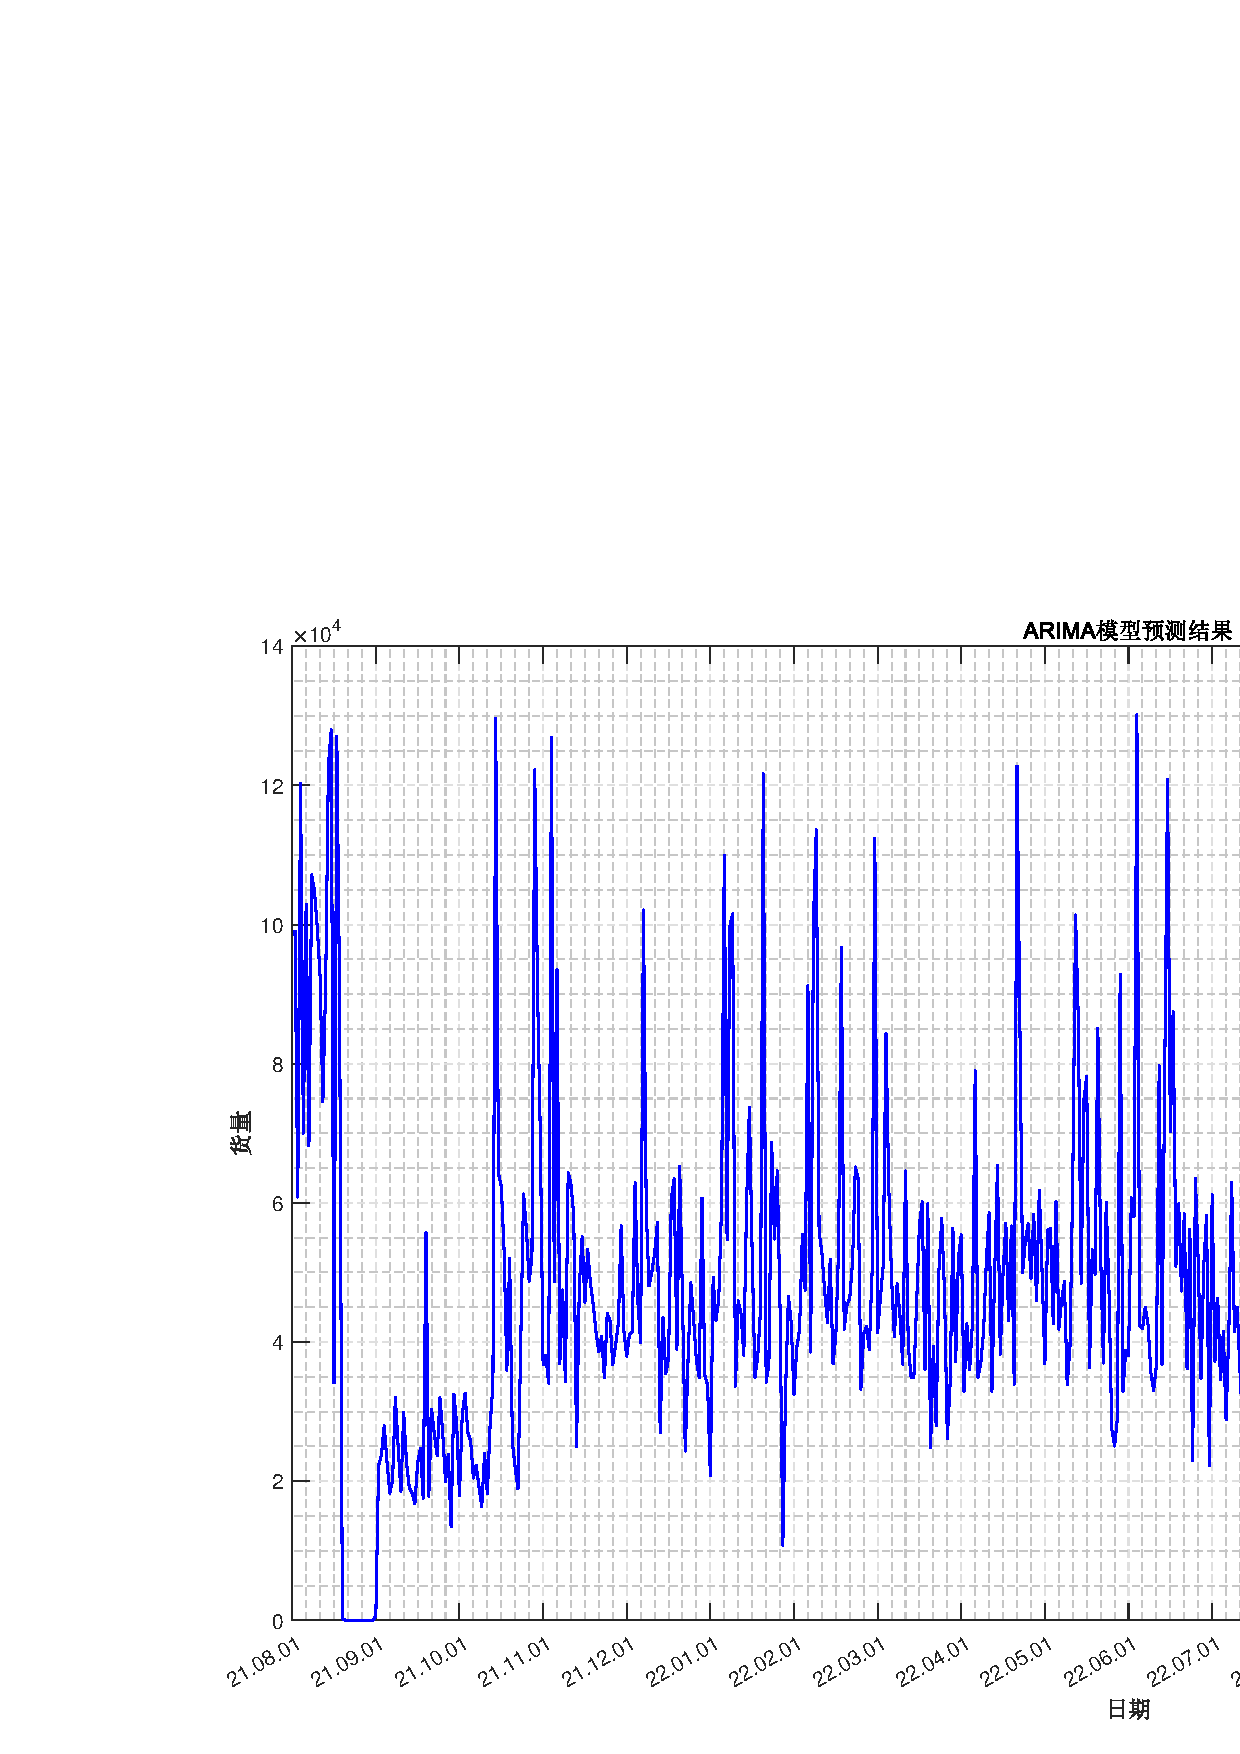
\includegraphics[width=\textwidth]{figure/1.pdf}
		\caption{线路$DC14\to DC10$的预测结果}\label{arima}
	\end{figure}

在这里我们利用$ARIMA$模型对每条线路的数据都做出了较好的预测,我们在这里列出$DC14\to DC10,DC20\to DC35,DC25\to DC62$这三条路线在2023.01.01-2020.01.31这三十天的预测结果,我们将它展示在表\ref{a}中:
\begin{table}[h]
\centering
\caption{各线路预测结果}
\label{a}
\begin{tabular}{cccc}
\hline
日期 & $DC14\to DC10$ & $DC20\to DC35$ & $DC25\to DC62$ \\ \hline
2023-01-01             & 26708    & 175    & 12065     \\
2023-01-02             & 39045    & 196    & 12677    \\
2023-01-03             & 40213    & 82    & 13286    \\
2023-01-04             & 31040     & 180    & 12234    \\
2023-01-05             & 29088    & 80    & 16000   \\
2023-01-06             & 33765    & 132    & 14852    \\
2023-01-07             & 28966   & 206    & 7670    \\
2023-01-08             & 29023    & 210   & 13309    \\
2023-01-09             & 35513    & 289   & 11806    \\
2023-01-10             & 35169    & 138    & 14365    \\
2023-01-11             & 29288     & 293    & 12840    \\
2023-01-12             & 23056    & 163    & 7071    \\
2023-01-13             & 22169   & 160    & 10255    \\
2023-01-14             & 17325   & 134    & 15325    \\
2023-01-15             & 19791     & 335    & 15942    \\
2023-01-16             & 20197   & 92     & 12475    \\
2023-01-17             & 20029   & 225    & 14364    \\
2023-01-18             & 19590    & 40    & 10956    \\
2023-01-19             & 19444    & 148   & 10041    \\
2023-01-20             & 22859   & 97    & 11046    \\
2023-01-21             & 22515    & 237    & 9466     \\
2023-01-22             & 22565    & 145     & 5451    \\
2023-01-23             & 24511    & 259   & 8694    \\
2023-01-24             & 23252    & 152    & 13189    \\
2023-01-25             & 21596    & 256    & 13297    \\
2023-01-26             & 25445    & 147    & 10705    \\
2023-01-27             & 24037    & 226    & 9410    \\
2023-01-28             & 22937    & 140   & 10653    \\
2023-01-29             & 24033    & 237    & 4241    \\
2023-01-30             & 22738    & 134    & 9722    \\ \hline
\end{tabular}
\end{table}

\section{问题2的模型建立与求解}
\subsection{规划模型的建立}
我们列出约束条件和目标函数,利用启发式算法求解,这样我们可以得到尽可能均衡的载货量、尽可能变化少的站点以及尽可能少的不能正常流转的货物。

根据我们第一问的预测,在站点$DC5$能够正常工作时,站点$D$在第$k$天时发出的货物量为$S_D\_k$,接受的货物量为$F_D\_k$。其中$D$为因$DC5$关停而导致变化的站点,$1\le k\le 30$(2023.01.01为第1天,2023.01.30为第30天),站点$DC5$在第$k$天时发出的包裹量为$F_{DC5}\_k$,接收的包裹量为$S_{DC5}\_k$。因$DC5$关停导致发生变化的站点数量为$x_D$,站点$D$的最大发出量为$F_{D_m}$,最大接收量为$S_{D_m}$,我们定义站点$D$在第$k$天的工作负荷计算如下:
\begin{eqnarray}
w_D\_k=\frac{1}{2}(\frac{S'_D\_k}{S_{D_m}}+\frac{F'_D\_k}{F_{D_m}})\times100\%,0\le w_D\_k\le 1
\end{eqnarray}
\begin{eqnarray}
\left\{\begin{matrix}
 S_D'\_k=S_D\_k+\Delta S_D\_k,S'_D\_k\le S_{D_m} \\
  F_D'\_k=F_D\_k+\Delta F_D\_k,F'_D\_k\le F_{D_m}
\end{matrix}\right.
\end{eqnarray}
其中,$w_D\_k$表示站点$D$在第$k$天时的工作负荷,$\Delta S_D\_k$表示在第$k$天时站点$D$需额外接收的货物量,$\Delta F_D\_k$表示在第$k$天时站点$D$需额外发出的货物量。$S'_D\_k$表示改变后站点$D$在第$k$天时的总接收量,$F'_D\_k$表示改变后站点$D$在第$k$天时的总发出量。

又因为站点$D$在第$k$天时的发出量和接收量均不超过当天站点$DC5$的日累计总量:
\begin{eqnarray}
\left\{\begin{matrix}
 \sum\limits_D\Delta S_D\_k\le S_{DC5}\_k+\sum\limits_{i=1}^{k-1}(S_{DC5}\_i-\sum\limits_D\Delta S_{D}\_i) \\
  \sum\limits_D\Delta F_D\_k\le F_{DC5}\_k+\sum\limits_{i=1}^{k-1}(F_{DC5}\_i-\sum\limits_D\Delta F_{D}\_i)
\end{matrix}\right.
\end{eqnarray}

日累计总量计算如下:
\begin{eqnarray}
SR=\sum\limits_{k}(F_{DC5}\_k+S_{DC5}\_k)-\sum\limits_k\sum\limits_D(\Delta F_{D}\_k+\Delta S_{D}\_k)
\end{eqnarray}

我们计算站点$D$在第$k$天时的工作负荷的方差$DX\_k$如下:
\begin{eqnarray}
DX\_k=\frac{1}{x_D}\sum\limits_D(w_D\_k-\frac{1}{x_D}\sum\limits_Dw_D\_k)^2
\end{eqnarray}

为了让各站点工作负荷尽可能均衡,我们有:
\begin{eqnarray}
\min \  \sum\limits_kDX\_k
\end{eqnarray}

为了使站点变化数量尽可能少,我们有:
\begin{eqnarray}
\min \ x_D
\end{eqnarray}

为了使货物尽可能正常流转,即日累计总量尽可能少,我们有:
\begin{eqnarray}
\min \ SR
\end{eqnarray}
\subsection{$FNS$方法介绍}
$FNS$(Fast Normalized Normal Constraint)方法是一种将多目标规划($MOP$)问题转化为单目标规划($SOP$)问题的方法。在这种方法中,使用归一化技术将多个目标函数组合为一个单一的函数,使得目标函数的最小值等价于原始多目标规划问题的最优解。具体来说,假设我们有一个$MOP$问题,其中有$m$个目标函数:

\begin{equation}
\begin{aligned}
\min \ \quad &\vec{f}(\vec{x})=(f_1(\vec{x}),f_2(\vec{x}),\dots,f_m(\vec{x})),&\vec{x}\in X
\end{aligned}
\end{equation}

其中,$\vec{x}=(x_1,x_2,\dots,x_n)$是决策变量向量,$X$是决策变量的可行域。FNS方法的目标是将多个目标函数合并为一个单一的函数$F(\vec{x})$,使得问题变为:

\begin{equation}
\begin{aligned}
\min \ \quad &F(\vec{x})=\frac{1}{m}\sum_{i=1}^{m} \frac{f_i(\vec{x})-f_iX}{f_iX-f_i^*(\vec{x})}, &\vec{x}\in X
\end{aligned}
\end{equation}

其中,$f_iX$表示目标函数$f_i$在可行域$X$中的最小值,$f_i^*(\vec{x})$表示目标函数$f_i$在当前解$\vec{x}$处的函数值。可以看出,$F(\vec{x})$是归一化的目标函数,它考虑了每个目标函数的贡献,并对每个目标函数进行了归一化,以便它们可以直接组合在一起。此外,由于$FNS$方法将多个目标函数合并为一个,所以问题变为了一个单目标规划问题,可以使用单目标优化算法来解决。

$FNS$方法的优点是可以将$MOP$问题转化为一个等价的$SOP$问题,这样可以更容易地使用单目标优化算法进行求解。但是$FNS$方法可能存在精度损失问题,因为它将多个目标函数合并为一个。
% 对于以上三个目标函数,我们分别加以权重$W_1,W_2,W_3$:
% \begin{eqnarray}
% 	W_1+W_2+W_3=1
% \end{eqnarray}

% 于是我们得到了我们最终的目标函数:
% \begin{eqnarray}
% \min \ W_1\cdot \sum\limits_kDX\_k+W_2\cdot x_D+W_3\cdot SR
% \end{eqnarray}
\subsection{问题2的求解}
我们的问题规模较大,几乎不能利用常规方法求解,所以我们采用寻优算法来寻找较优解。机器寻优(Machine Learning Optimization)是指为了优化机器学习模型的性能而进行的一系列算法和技术。机器寻优算法的目标是找到模型的最优参数组合,以最小化模型在测试数据上的误差或者最大化模型的性能指标。我们在这里采用遗传算法来进行求解。
\subsubsection{遗传算法介绍}
遗传算法是一种模拟自然界生物进化过程的计算方法,它是一种基于群体并行搜索的随机优化算法。遗传算法通常用于求解优化问题,如函数优化、组合优化、序列优化等。

遗传算法可以被用来寻找最优的货物分配方案。具体来说,遗传算法通过模拟生物进化过程中的基因遗传、交叉、变异等过程来生成一组优秀的解决方案。每个解决方案由一组基因表示,而每个基因又表示为一种分配方式。

在遗传算法的迭代过程中,算法会评估每个解决方案的适应度,即其与问题目标的匹配程度。适应度高的解决方案将有更高的概率在下一代中被选择并进行交叉、变异等操作,从而产生新的解决方案。这个过程将一直持续到达到某个停止准则,如达到最大迭代次数或找到最优解等。由于遗传算法的并行处理方式,它可以有效地处理大规模的问题。
\subsubsection{遗传算法寻优}
对于我们的目标函数,当站点$DC5$正常运转时,我们的目标函数能够达到最小值为0,当站点$DC5$停运时,我们将$DC5$包裹均匀分配到所有路线上,得到我们的初始解,此时我们目标函数达到最大值为3。
接下来我们利用遗传算法进行求解,得出最终的目标函数能够达到全局较优解使目标函数值达到1.161。我们求得的最优分配方案使得未能正常流转的货物量为0,改变的线路及货量和改变后线路的平均负荷率展示在表\ref{wt2}中,遗传算法求解目标函数最小值展示在图\ref{yichuan}:
\begin{table}[h]
\centering
\caption{问题2结果}
\label{wt2}
\begin{tabular}{lcc}
\hline
改变的线路&	新增的货量&	改变后线路平均负荷率 \\ \hline
$DC14\to DC8 $   & 285169  & 100$\%$  \\
$DC14\to DC9$  & 223279   & 100$\%$ \\
$DC36\to DC4$   & 85168  & 99.7$\%$  \\
$DC23 \to DC4$  & 61498   & 99.4$\%$ \\
$DC23\to DC10$  & 23157    &99.6$\%$\\\hline
\end{tabular}
\end{table}
\begin{figure}[H]
		\centering
		\includegraphics[width=\textwidth]{figure/3.pdf}
		\caption{遗传算法求得的最优解}\label{yichuan}
	\end{figure}




















\newpage
\section{问题3的模型建立与求解}
\subsection{问题3模型的建立}
问题3需要我们在站点$DC9$被关停后,对物流网络进行动态调整,我们首先列出约束条件和目标函数再利用寻优算法来求解。

我们设各站点所构成的集合为$D$,路线$D_i\to D_j$记为$L_{D_iD_j}$。根据我们第一问的预测,在站点$DC9$正常工作时,所有的路线集合记为$V_D$,在$DC9$停运后第$k$天的所有路线集合记为$V_L\_k$,在第$k$天因$DC9$停运而引起改变的所有路线集合记为$V_G\_k$,我们有:
\begin{eqnarray}
V_G\_k=(V_D\cup V_L\_k)/(V_D\cap V_L\_k)
\end{eqnarray}

在$DC9$停运第$k$天时运行并且停运前也正常运行的线路集合记为$V_{both}\_k$,我们有:
\begin{eqnarray}
V_{both}\_k=V_D\cap V_L\_k
\end{eqnarray}

在第$k$天关停的路线集合记为$V_{off}\_k$,我们有:
\begin{eqnarray}
V_{off}\_k=V_D/(V_D\cap V_L\_k)
\end{eqnarray}

在第$k$天新开的路线集合记为$V_{on}\_k$,我们有:
\begin{eqnarray}
V_{on}\_k=V_L/(V_D\cap V_L\_k)
\end{eqnarray}

我们记路线$L_{D_iD_j}$在$DC9$关停前根据我们第一问的预测货量为$H_{L_{D_iD_j}}\_k$,在$DC9$关停后的货量为$H'_{L_{D_iD_j}}\_k$,分配到的货量为$\Delta H_{L_{D_iD_j}}\_k(\Delta H_{L_{D_iD_j}}\_k\ge 0)$,新开路线的最大货量为$H_{max}$,在$DC9$关停后,我们有:
\begin{eqnarray}
H'_{L_{D_iD_j}}\_k=\left\{\begin{matrix}
 \Delta H_{L_{D_iD_j}}\_k&L_{D_iD_j}\_k\in V_{on}\_k \\
  0&L_{D_iD_j}\_k\in V_{off}\_k \\
  H_{L_{D_iD_j}}\_k+\Delta H_{L_{D_iD_j}}\_k&L_{D_iD_j}\_k\in V_{both}\_k
\end{matrix}\right.
\end{eqnarray}

其中,$H'_{L_{D_iD_j}}\_k$取值范围为:
\begin{eqnarray}\left\{\begin{matrix}
0\le H'_{L_{D_iD_j}}\_k\le H_{max}&,L_{D_iD_j}\_k\in V_{on}\_k\\ 
H_{L_{D_iD_j}}\_k\le H'_{L_{D_iD_j}}\_k\le \max \ \bigcup\limits_{k}H_{L_{D_iD_j}}\_k&,L_{D_iD_j}\_k\in V_{both}\_k\end{matrix}\right.
\end{eqnarray}

设第$k$天由路线$L_{D_iDC9}\_k$改为的路线$L_{D_iD_j}\_k$所有路线集合为$V_{D_iDC9}\_k$,由路线$L_{DC9D_j}\_k$改为的路线$L_{D_iD_j}\_k$所有路线集合为$V_{DC9D_j}\_k$,又分配总量不超过当天日累计总量$SR$,则有:
\begin{eqnarray}
\left\{\begin{matrix}
\sum\limits_{V_{D_iDC9}\_k}\Delta H_{L_{D_iD_j}}\_k\le \sum\limits_{n=1}^k\sum\limits_{V_D}H_{L_{D_iDC9}}\_n-\sum\limits_{n=1}^{k-1}\sum\limits_{V_D}\Delta H_{L_{D_iDC9}}\_n
\\
\sum\limits_{V_{DC9D_j}\_k}\Delta H_{L_{D_iD_j}}\_k\le \sum\limits_{n=1}^k\sum\limits_{V_D}H_{L_{DC9D_j}}\_n-\sum\limits_{n=1}^{k-1}\sum\limits_{V_D}\Delta H_{L_{DC9D_j}}\_n
\end{matrix}\right.
\end{eqnarray}

日累计总量计算如下:
\begin{eqnarray}
SR=\sum\limits_k\sum\limits_{V_D}(H_{L_{D_iDC9}}\_k+H_{L_{DC9D_j}}\_k)-\sum\limits_k\sum\limits_{V_{D_iDC9}\_k}\sum\limits_{V_{DC9D_j}\_k}\Delta H_{L_{D_iD_j}}\_k
\end{eqnarray}

最小的日累计总量有:
\begin{eqnarray}
\min \ SR
\end{eqnarray}

设改变的线路数为$Change,\mathop{\text{card}}\limits_P\ A$表示在约束条件$P$下集合$A$中元素个数,则我们有:
\begin{eqnarray}
Change=\sum\limits_k(\mathop{\text{card}}\ V_{G}\_k+\mathop{\text{card}}\limits_{\Delta H_{L_{D_iD_j}}\_k>0}\ V_{D}\_k)
\end{eqnarray}

最少的改变线路数有:
\begin{eqnarray}
\min \ Change
\end{eqnarray}

我们设线路$L_{D_iD_j}$在第$k$天时的负荷量为$w_{L_{D_iD_j}}\_k$计算如下:
\begin{eqnarray}
w_{L_{D_iD_j}}\_k=\left\{\begin{matrix}
 \frac{H_{L_{D_iD_j}}\_k}{H_{max}} &L_{D_iD_j}\_k\in V_{on}\_k\\
  0&L_{D_iD_j}\_k\in V_{off}\_k \\
  \frac{H'_{L_{D_iD_j}}\_k}{\max \ \bigcup\limits_{k}H_{L_{D_iD_j}}\_k}& L_{D_iD_j}\_k\in V_{both}\_k
\end{matrix}\right.\times 100\%
\end{eqnarray}

第$k$天各路线负荷量方差为$DX\_k$计算如下:
\begin{eqnarray}
DX\_k=\frac{1}{{\text{card}}\ V_{L}\_k}\sum\limits_{V_{L}\_k}(w_{L_{D_iD_j}}\_k-\frac{1}{{\text{card}}\ V_{L}\_k}\sum\limits_{V_{L}\_k}w_{L_{D_iD_j}}\_k)^2
\end{eqnarray}

为了使各路线负荷量尽可能均衡,我们有:
\begin{eqnarray}
\min \ \sum\limits_{k}DX\_k
\end{eqnarray}

% 我们对以上三个目标函数分别加以权重$W_1',W_2',W_3'$:
% \begin{eqnarray}
% W_1'+W_2'+W_3'=1
% \end{eqnarray}

% 于是我们得到了我们最终的目标函数:
% \begin{eqnarray}
% \min \ W_1'\cdot \sum\limits_kDX\_k+W_2'\cdot Change +W_3'\cdot SR
% \end{eqnarray}
对于以上三个目标函数,我们仍利用FNS方法转化为一个目标函数。但是需要注意的是,我们在利用FNS将多目标函数转化为单目标函数后我们得到的是极小型目标函数,为了方便后续的求解我们在转化后的目标函数前加上负号使得我们算法求解的目标函数为极大型的目标函数。
\subsection{问题3模型的求解}
量子遗传算法(Quantum Genetic Algorithm,QGA)是量子计算和遗传算法相结合的一种优化算法。它将传统遗传算法的进化和选择过程应用于量子比特,以在优化问题中搜索最优解。在遗传算法的基础上,我们引入QGA来进行问题3的求解。
\subsubsection{量子遗传算法介绍}
QGA是一种基于量子比特的遗传算法,它利用量子态的叠加和纠缠特性,实现在优化问题中搜索最优解的目的。

QGA的基本思想是利用量子比特的叠加和纠缠特性,在量子状态空间中搜索最优解。它通过三个基本的操作:量子叠加、量子旋转和量子测量来实现。

首先,将一个初始种群表示为一个量子态 $|\psi\rangle$。然后,使用量子叠加操作,将其变成一个均匀叠加态:
\begin{eqnarray}
|\psi\rangle=\frac{1}{\sqrt{N}}\sum_{i=1}^{N}|x_i\rangle
\end{eqnarray}
其中,$N$ 是种群中的个体数量,$|x_i\rangle$ 表示第 $i$ 个个体的状态。

接下来,使用量子旋转门 $R$,将量子态旋转到目标态 $|\phi\rangle$。这个目标态是通过适应度函数计算得到的:
\begin{eqnarray}
|\phi\rangle=\sum_{i=1}^{N}\sqrt{p_i}|x_i\rangle
\end{eqnarray}
其中,$p_i$ 是第 $i$ 个个体的适应度值。旋转门 $R$ 的定义为:

\begin{eqnarray}
R=\left ( \begin{matrix}
 \cos\theta  &-\sin\theta  \\
  \sin\theta&\cos\theta 
\end{matrix} \right ) 
\end{eqnarray}
其中,$\theta$ 是旋转角度。为了最大化目标函数,旋转角度可以设置为:
\begin{eqnarray}
\theta=2\arcsin\sqrt{p_i}
\end{eqnarray}

最后,使用量子测量将量子态转化为经典的个体,得到下一代种群。重复执行上述步骤,直到找到最优解或达到预定的迭代次数。
\subsubsection{量子遗传算法寻优}
对于我们的目标函数,当站点$DC9$正常运行时,我们的目标函数能够达到最大值为0,在站点$DC9$停运后,我们将与$DC9$相关路线包裹平均分配到每条路线上并且不新开线路也不进行动态调整,此时目标函数取得最小值为-3。在此基础上我们利用量子遗传算法进行求解,得出最终目标函数的最大值达到-1.15,目标函数平均最大值也能达到-1.15。在第2,3,8,9天新开路线$DC14\to DC28$,其余时间没有新开或关闭路线,没有未能流转的包裹量。我们改变的线路及货量和改变后线路平均负荷率展示在表\ref{dc9},量子遗传算法求解目标函数最大值展示在图\ref{lzycsf}中:
% \begin{table}[h]
% \centering
% \caption{问题3结果}
% \label{dc9}
% \begin{tabular}{lcc}
% \hline
% 改变的线路&	新增的货量&	改变后线路平均负荷率 \\ \hline
% $DC14\to DC28$(新开路线)&72995976&100$\%$\\
% $DC14\to DC8 $   & 185169  & 100$\%$  \\
% $DC14\to DC28$  & 124356   & 100$\%$ \\
% $DC36\to DC4$   & 83242  & 98.4$\%$  \\\hline
% \end{tabular}
% \end{table}
\begin{table}[!h]
    \caption{问题3结果}
\label{dc9}
    \centering
    \begin{threeparttable}          %这行要添加
      \begin{tabular}{lcc}
\hline
改变的线路&	新增的货量&	改变后线路平均负荷率 \\ \hline
$DC14\to DC28$\tnote{1}&72995976&100$\%$\\
$DC14\to DC8 $   & 185169  & 100$\%$  \\
$DC14\to DC28$  & 124356   & 100$\%$ \\
$DC36\to DC4$   & 83242  & 98.4$\%$  \\\hline
\end{tabular}
         \begin{tablenotes}    %这行要添加, 从这开始
        \footnotesize               %这行要添加
        \item[1] 该路线为新增路线,仅在第2、3、8、9天运行。
      \end{tablenotes}            %这行要添加
    \end{threeparttable}       %这行要添加,到这里结束
  \end{table}
\begin{figure}[h]
		\centering
		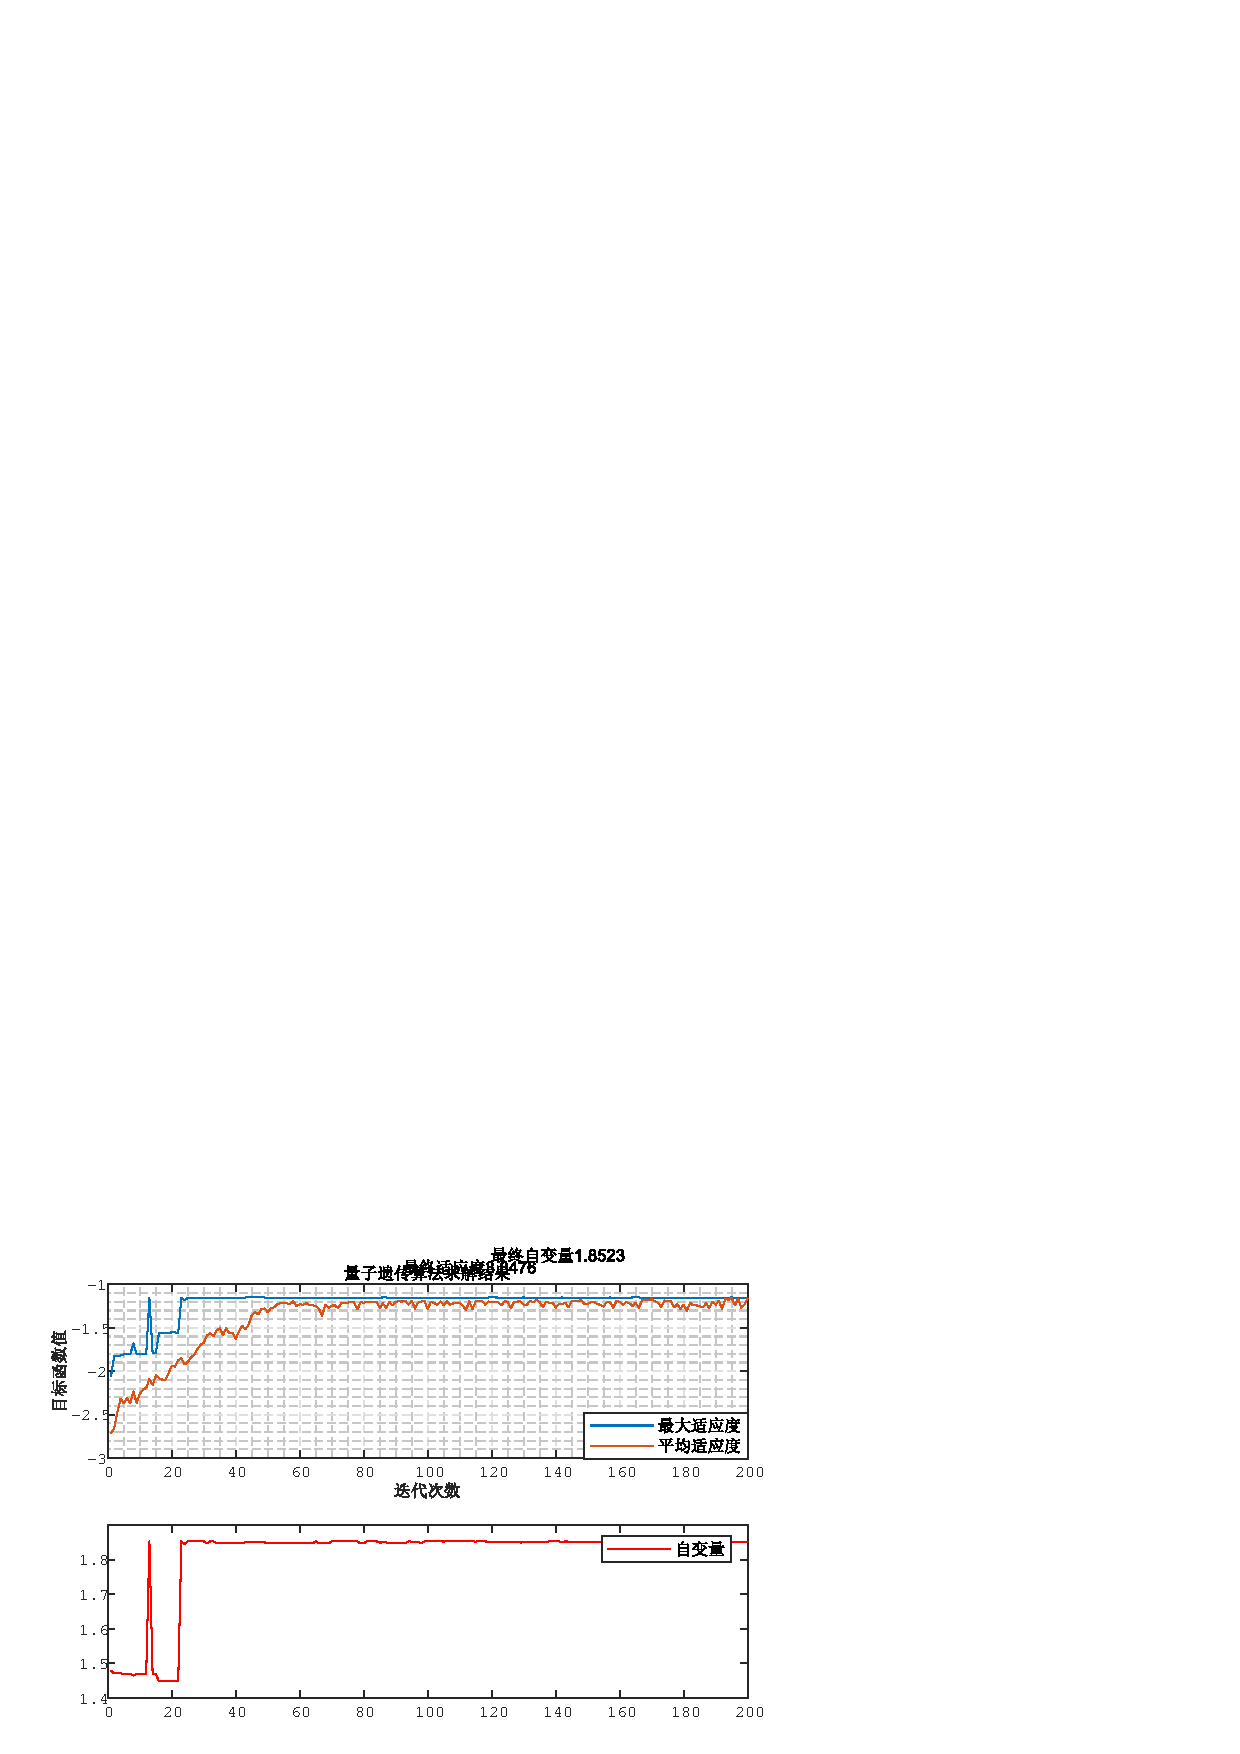
\includegraphics[width=\textwidth]{figure/4.pdf}
		\caption{量子遗传算法求得的最优解}\label{lzycsf}
	\end{figure}
% \begin{table}[h]
%     \centering
%     \begin{tabular}{lcc}
% \hline
% 改变的线路&	新增的货量&	改变后线路平均负荷率 \\ \hline
% $DC14\to DC28$&72995976&100$\%$\\
% $DC14\to DC8 $   & 185169  & 100$\%$  \\
% $DC14\to DC28$  & 124356   & 100$\%$ \\
% $DC36\to DC4$   & 83242  & 98.4$\%$  \\\hline
% \end{tabular}

%     \caption{问题3结果}
% \label{dc9}
% \end{table}










% FNS(Fast Normalized Normal Constraint)方法是一种将多目标规划(MOP)问题转化为单目标规划(SOP)问题的方法。在这种方法中,使用归一化技术将多个目标函数组合为一个单一的函数,使得目标函数的最小值等价于原始多目标规划问题的最优解。具体来说,假设我们有一个MOP问题,其中有$m$个目标函数:

% \begin{equation}
% \begin{aligned}
% \text{minimize}\quad &\vec{f}(\vec{x})=(f_1(\vec{x}),f_2(\vec{x}),\dots,f_m(\vec{x}))\
% \text{subject to}\quad &\vec{x}\in X,
% \end{aligned}
% \end{equation}

% 其中,$\vec{x}=(x_1,x_2,\dots,x_n)$是决策变量向量,$X$是决策变量的可行域。FNS方法的目标是将多个目标函数合并为一个单一的函数$F(\vec{x})$,使得问题变为:

% \begin{equation}
% \begin{aligned}
% \text{minimize}\quad &F(\vec{x})=\frac{1}{m}\sum_{i=1}^{m} \frac{f_i(\vec{x})-f_i^(X)}{f_i^(X)-f_i^*(\vec{x})}\
% \text{subject to}\quad &\vec{x}\in X,
% \end{aligned}
% \end{equation}

% 其中,$f_i^(X)$表示目标函数$f_i$在可行域$X$中的最小值,$f_i^(\vec{x})$表示目标函数$f_i$在当前解$\vec{x}$处的函数值。可以看出,$F(\vec{x})$是归一化的目标函数,它考虑了每个目标函数的贡献,并对每个目标函数进行了归一化,以便它们可以直接组合在一起。此外,由于FNS方法将多个目标函数合并为一个,所以问题变为了一个单目标规划问题,可以使用单目标优化算法来解决。

% FNS方法的优点是可以将MOP问题转化为一个等价的SOP问题,这样可以更容易地使用单目标优化算法进行求解。此外,FNS方法不需要任何权重向量或任何先验知识,因此更加灵活和通用。但是,FNS方法可能存在精度损失问题,因为它将多个目标函数合并为一个。因此,在使用FNS方法时,需要注意解的精度是否满足要求。

















\clearpage
\section{问题4的求解}
\subsection{熵权法介绍}
熵权法是一种常用的多指标权重确定方法,它可以将指标之间的相关性考虑进来,避免了传统加权平均方法中的主观性和不确定性,有效地考虑指标之间的相关性,避免传统加权平均方法中的主观性和不确定性。

其基本思想是将指标之间的熵值作为权重,越重要的指标熵值越小,从而实现对指标的优先排序和加权。运用熵权法我们就客观的得到了物流线路的重要性排序。
\subsection{重要性求解}
对物流场地和物流路线的重要性评价。对于物流线路重要性的分析,我们认为如果一条物流线路的货量越大,这条物流线路越重要;同理若这条线路负荷量越大,重要性也越高。于是我们对数据处理后进行分析,找到货量较高的一些站点再运用熵权法进行评分得到各线路重要性排序。对于物流场地而言,我们简单认为处理的平均货量越大则站点越重要。我们将得出的最重要的十条路线和十个站点展示在表\ref{xlzyx}和表\ref{zyx}中:

% \subsubsection{物流路线重要性排序}
% \begin{table}[h]
% \centering
% \caption{线路重要性排名}
% \label{xlzyx}
% \begin{tabular}{lc}
% \hline
% 线路      & 重要性排名 \\ \hline
% $DC14\to DC8 $   & 1     \\
% $DC14\to DC9$  & 2     \\
% $DC36\to DC10$   & 3     \\
% $DC23 \to DC4$  & 4     \\
% $DC23\to DC10$  & 5     \\
% $DC19\to DC4$  & 6     \\
% $DC17\to DC4 $ & 7     \\
% $DC22\to DC10$  & 8     \\
% $DC24\to DC3$   & 9     \\
% $DC10\to DC23$  & 10    \\ \hline
% \end{tabular}

% \end{table}
% % \subsubsection{物流场地重要性排序}
% \begin{table}[h]
% \centering
% \caption{站点重要性排名}
% \label{zyx}
% \begin{tabular}{lcc}
% \hline
% 站点      & 平均货运量       & 重要性排名 \\ \hline
% $DC14$    & 360728 & 1     \\
% $DC10  $& 359481 & 2     \\
% $DC4$   & 305181  & 3     \\
% $DC8 $  & 257334  & 4     \\
% $DC62$ & 123824 & 5     \\
% $DC23$ & 101918 & 6     \\
% $DC36 $ & 100918  & 7     \\
% $DC17 $ & 96090 & 8     \\
% $DC9 $  & 94691 & 9     \\
% $DC19$ & 89820 & 10    \\ \hline
% \end{tabular}
% \end{table}



\begin{table*}[h]
\begin{floatrow}
\capbtabbox{
\begin{tabular}{lc}
\hline
线路      & 重要性排名 \\ \hline
$DC14\to DC8 $   & 1     \\
$DC14\to DC9$  & 2     \\
$DC36\to DC10$   & 3     \\
$DC23 \to DC4$  & 4     \\
$DC23\to DC10$  & 5     \\
$DC19\to DC4$  & 6     \\
$DC17\to DC4 $ & 7     \\
$DC22\to DC10$  & 8     \\
$DC24\to DC3$   & 9     \\
$DC10\to DC23$  & 10    \\ \hline
\end{tabular}
}{
\caption{线路重要性排名}
\label{xlzyx}
}
\capbtabbox{
\begin{tabular}{lcc}
\hline
站点      & 平均货运量       & 重要性排名 \\ \hline
$DC14$    & 360728 & 1     \\
$DC10  $& 359481 & 2     \\
$DC4$   & 305181  & 3     \\
$DC8 $  & 257334  & 4     \\
$DC62$ & 123824 & 5     \\
$DC23$ & 101918 & 6     \\
$DC36 $ & 100918  & 7     \\
$DC17 $ & 96090 & 8     \\
$DC9 $  & 94691 & 9     \\
$DC19$ & 89820 & 10    \\ \hline
\end{tabular}
}{
 \caption{站点重要性排名}
\label{zyx}
 \small
}
\end{floatrow}
\end{table*}














\subsection{新增物流路线的确定}
对于新增的物流场地应该与哪几个已有物流线路之间新增路线,我们首先应当考虑与物流量大的线路和负荷率高的线路,这样可以有效的降低高负荷高货量的物流线路的压力,也能减轻一些物流站点的所需的处理货量的压力。根据我们对各物流线路和场地的评价,注意到站点$DC14,DC10$和$DC4$三个站点的货量压力很大,同时与它们相关的线路也很重要。我们新增的站点应当与这三个站点间建立联系。又注意到线路集合$L_{DC14D_j}$中有两条很重要的线路$DC14\to DC8,DC14\to DC9$。这两条线路如果出现故障对于站点$DC14$的压力将会大大增加,所以我们的第一条线路就应当是在这两条路线出现故障时能够有效缓解该站点的压力。假设我们新建立的站点为$DCX$,我们的第一对路线就是$DCX\to DC14$和$DC14\to DCX$。

通过上述分析,我们紧接着注意到两个路线集合$L_{DC_iDC10}$和$L_{DC_iDC4}$,所以我们的剩下两对路线就随之确定了,分别为$DC10\to DCX,DCX\to DC10$和$DC4\to DCX,DCX\to DC4$。接下来我们还需考虑该站点的处理能力和新增路线的运输能力。
\subsection{新增站点和线路的能力设置}
对于新建站点的处理能力,在不新增这个站点时物流网络能够正常运行,所以我们对该物流站点的处理能力似乎不需要太过担心。但是它又同时连接了三条最重要的站点,正如上面所说,在其中任意一个站点发生故障的情况下,我们都应当利用这个新增的站点来减轻我们物流网络的负荷并且保证包裹尽可能正常流转。这也同时能够保证更少的物流线路发生改变,所以我们的这个物流站点至少应该有三个站点中一个的处理能力—保证始终能够有三个最重要的站点在正常运行。我们通过附件一的数据得出这三个站点平均处理货量为341797,所以我们的站点$DCX$应该有负荷货量$341797$件的能力,四个站点均正常时每天也能够处理货量$256347$件。

对于新增路线的处理能力,如果运输能力太强,在三个站点均正常运行时,我们的物流路线就会造成资源的浪费;而如果运输能力太弱,若三个站点中有某个站点停运时,那么我们的新增路线就不能很好地应对这种情况,这与我们新增路线地初心相悖。这两种极端情况都是我们不愿意看到的,所以我们要在两者间取一个较优值对两种情况均能得到令人较为满意的结果。我们尝试在每年总货物量没有发生较大的突变的情况下使新增路线能够较好地融入原物流网络。又考虑到站点正常运行概率应该远远大于某站点停运的概率。于是我们让在四个站点均正常运行时重要的几条线路加上我们新增路线的负荷尽可能均衡。基于以上分析我们得到了新增路线的运输能力在表\ref{xz}中:
% Please add the following required packages to your document preamble:
% \usepackage{multirow}
\begin{table}[h]
\centering
\caption{新增路线的运输能力}
\label{xz}
\begin{tabular}{cccc}
\hline
\multirow{2}{*}{新增路线} & $DCX\to DC14$ & $DC10\to DCX$ & $DC4\to DCX$ \\ \cline{2-4} 
                      & $DC14\to DCX$ & $DCX\to DC10$ & $DCX\to DC4$ \\ \hline
运输能力                  & 27776         & 25815         & 22702        \\ \hline
\end{tabular}
\end{table}
\subsection{鲁棒性分析}
考虑到预测结果的随机性,我们需要对我们的物流网络结构进行鲁棒性分析。
\subsubsection{鲁棒性介绍}
鲁棒性是指系统或算法在面对输入数据中的不确定性、异常值、误差或攻击时的稳定性和可靠性。具有高鲁棒性的系统或算法能够在这些情况下仍能保持正确的输出或适当的行为。

鲁棒性对于许多应用是至关重要的,例如在金融、医疗、安全等领域,这些领域中的错误或异常值可能会导致重大的后果。在机器学习领域中,鲁棒性是一个重要的研究方向,因为许多机器学习算法在训练数据中的异常值、错误标签或攻击时可能会失效。
\subsubsection{具体分析}
我们对我们第1问线路$L_{D_iD_j}$在第$k$天预测的数据加上一个随机生成的扰动项$R_{L_{D_iD_j}}\_k$:
\begin{equation}
	|R_{L_{D_iD_j}}\_k|\le H_{L_{D_iD_j}}
\end{equation}
在我们的数据集加上这个随机扰动项观察我们的货物分配方案得到的目标函数值是否具有较大的波动。我们进行多次试验并将结果展示在图\ref{lbx}中:
\begin{figure}[h]
		\centering
		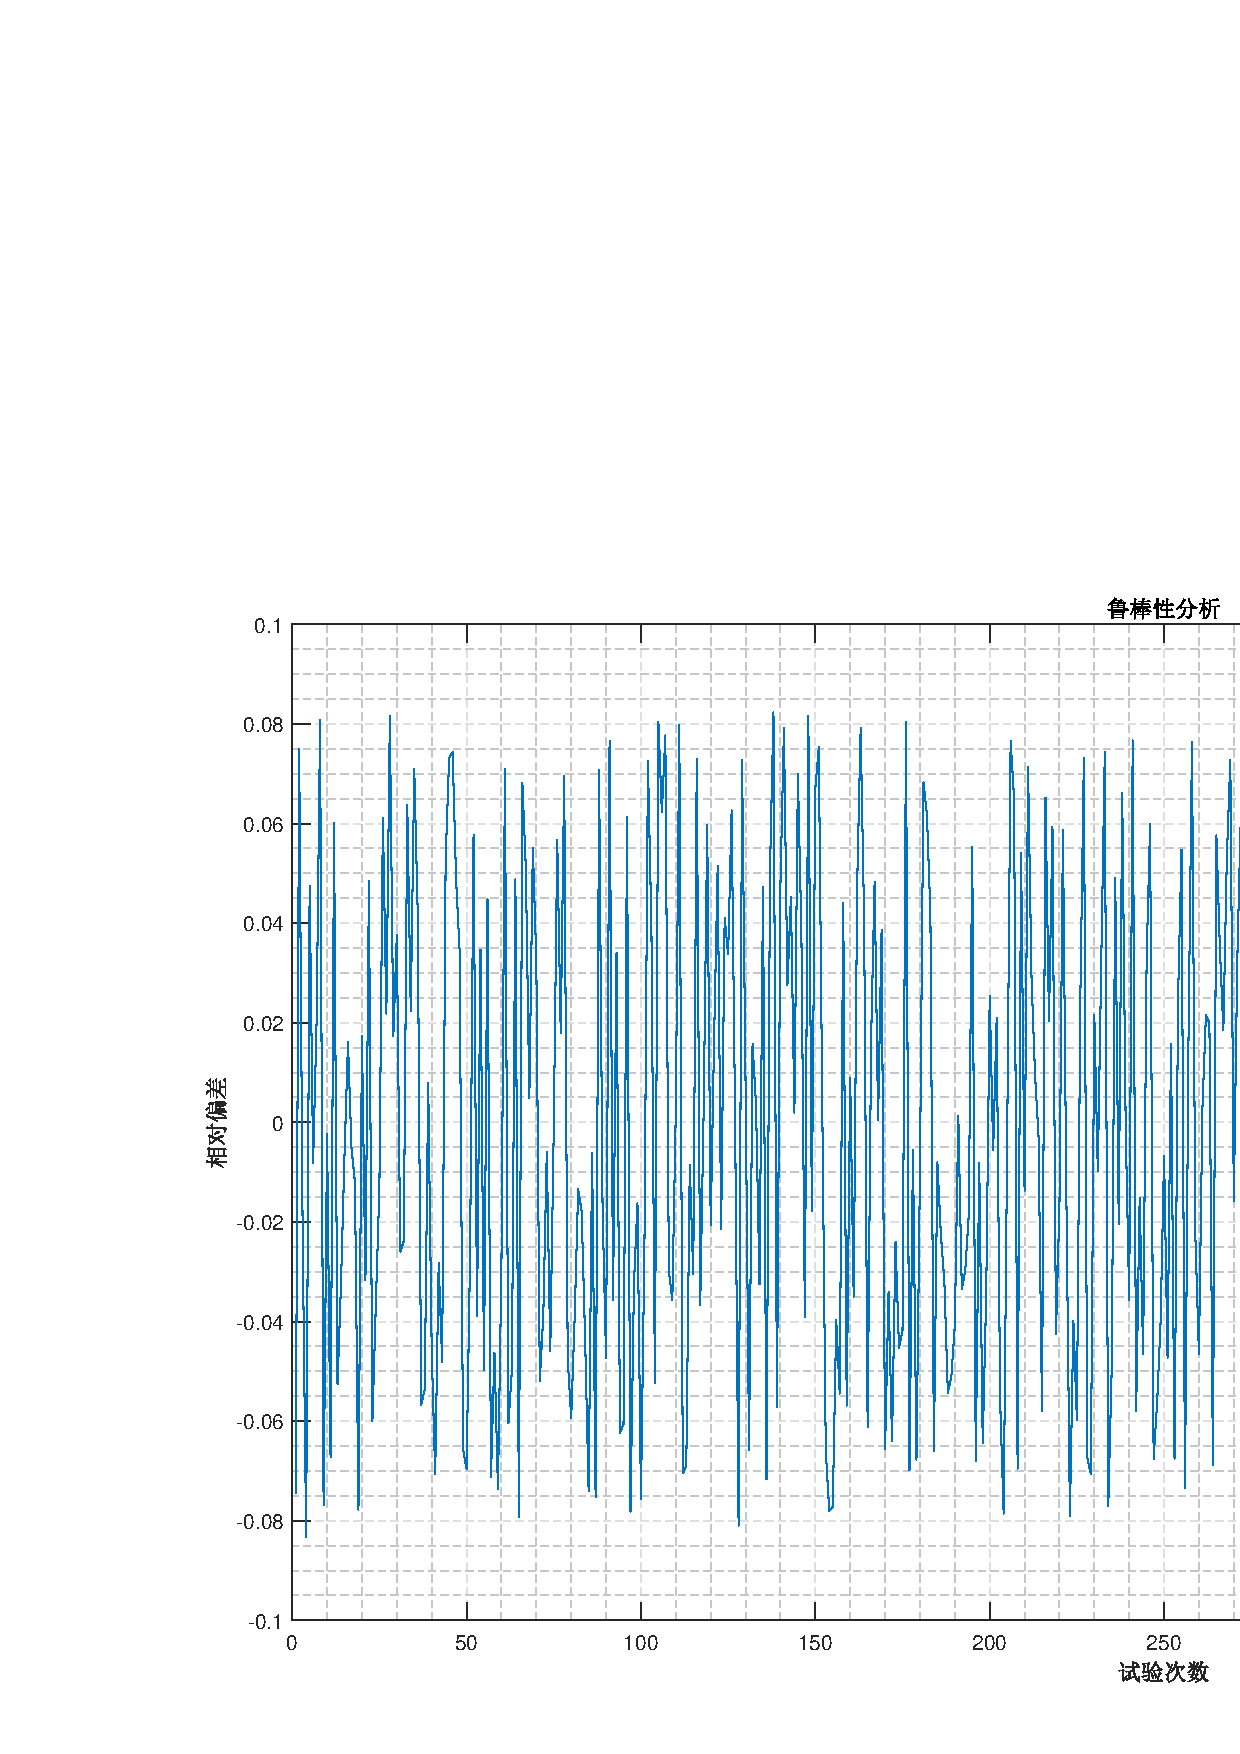
\includegraphics[width=\textwidth]{figure/5.pdf}
		\caption{鲁棒性分析}\label{lbx}
	\end{figure}

根据我们对数据的扰动,发现网络表现性能良好,最大偏差也不超过$10\%$,所以我们认为该物流网路鲁棒性较强。
	\newpage
% 	\subsection{模型的准备}

% 	\subsection{模型一的建立}
% 	效果见\cref{fig:1}。
% 	\begin{figure}[htbp]
% 		\centering
% 		\includegraphics{example-image-plain.pdf}
% 		\caption{content}\label{fig:1}
% 	\end{figure}
% 	\subsection{模型二的建立}
% 	结果见\cref{tab:1}。
% 	\begin{table}[htbp]
% 		\centering
% 		\caption{content}\label{tab:1}
% 		\begin{tabularx}{0.7\textwidth}{c@{\hspace{1pc}}|@{\hspace{2pc}}X}
% 		\Xhline{0.08em}
% 		符号 & \multicolumn{1}{c}{符号说明}\\
% 		\Xhline{0.05em}
% 		$\delta$ & 赤纬角\\
% 		$\beta$ & 经度\\
% 		$\alpha$ & 纬度\\
% 		$r$ & 地球半径\\
% 		$\gamma$ & 太阳光与杆所成的夹角\\
% 		$l$ & 杆的长度\\
% 		$l_{y}$ & 杆的影子长度\\
% 		$\vec{x}_{1},\vec{y}_{1},\vec{z}_{1}$ & 由杆的位置所生成的切平面的正交基\\
% 		$\vec{\hat{x}}_{1},\vec{\hat{y}}_{1},\vec{\hat{z}}_{1}$ & 由杆的位置所生成的切平面的单位正交基\\
% 		$\theta$ & 影子与北方的夹角\\
% 		$l_{y}(i)$ & 编号为 $i$ 的数据对应的影子长度\\
% 		$\theta_{i}$ & 编号为 $i$ 的数据对应的影子角度\\			\Xhline{0.08em}
% 		\end{tabularx}
% 	\end{table}
% 	\subsection{模型三的建立}
% 	\zhlipsum*[14]

% 	\section{模型的检验}
% 	\zhlipsum*[15]

	\section{模型评价}
	\subsection{模型的优点}
	\begin{enumerate}
		\item 在处理高维参数的优化问题中机器寻优算法具有良好的性能并且得到较优的结果。
		\item 机器寻优算法具有较强的鲁棒性,在存在噪声情况下仍能找到较好的优化解。
		\item 量子遗传算法对于我们复杂的优化问题具有更好的适应性。
	\end{enumerate}
	\subsection{模型的缺点}
	\begin{enumerate}
		\item 我们建立的$ARIMA$对于异常值较敏感,可能导致预测结果出现较大偏差。
		\item 我们用$FNS$方法将多个目标函数合并为一个可能存在精度损失问题。
		\item 在预测结果具有随机性的前提下我们的货量分配方案不具有普适性。
	\end{enumerate}

% 	\zhlipsum*[18]
% 	\subsection{模型的改进}
% 	\zhlipsum*[19]\cite{label}

	\phantomsection
	\addcontentsline{toc}{section}{参考文献}
	\begin{thebibliography}{99}
	\bibitem{__2015}
 宋树洋.
\newblock 改进遗传算法在应急物资调运模型中的应用.
\newblock {\em 科技视界}, (18):145--148, 2015.
\newblock 3 citations(CNKI)[2023-4-17].

\bibitem{__2015-1}
赵越.
\newblock {\em 区域性应急物流网络节点能力配置的研究}.
\newblock 硕士, 北京交通大学, 2015.
\newblock 3 citations(CNKI)[2023-4-17].
	\bibitem{c1} R. Wang, Y. Sun, and J. Zhang, “A hybrid quantum genetic algorithm for capacitated vehicle routing problem,” \emph{International Journal of Quantum Information}, vol. 17, no. 3, p. 1940001, 2019.

\bibitem{c2} G. Li, Z. Li, and M. Li, “A hybrid quantum-inspired genetic algorithm for multi-objective vehicle routing problem with time windows,” \emph{IEEE Access}, vol. 8, pp. 182064-182076, 2020.

\bibitem{c3} Y. Zhang, Y. Tang, and J. Yang, “Quantum-inspired genetic algorithm for multi-objective capacitated vehicle routing problem,” \emph{Journal of Advanced Transportation}, vol. 2020, p. 9563707, 2020.

\bibitem{c4} S. Chen, Y. Wu, and W. Zhang, “A quantum genetic algorithm for vehicle routing problem with time windows and multiple depots,” \emph{Journal of Advanced Transportation}, vol. 2019, p. 5850867, 2019.

\bibitem{c5} X. Zhang, H. Wu, X. Cheng, and C. Hu, “A quantum-inspired genetic algorithm for a location-routing problem with simultaneous pickup and delivery,” \emph{IEEE Access}, vol. 7, pp. 95366-95379, 2019.
	\end{thebibliography}

	\newpage
	\appendix

	\ctexset{section={
		format={\zihao{-4}\heiti\raggedright}
	}}
	\begin{center}
		\heiti\zihao{4} 附\hspace{1pc}录
	\end{center}
\section{ARIMA模型MATLAB 代码}
\begin{lstlisting}[language=Matlab]
% 自动选择 ARIMA 模型
Mdl = arima('D',1,'Seasonality',12,'MALags',1:12,'SMALags',1:12);
Mdl = estimate(Mdl, y);

% 模型诊断
res = infer(Mdl, y);
figure;
subplot(2,1,1)
plot(res);
title('模型残差')
subplot(2,1,2)
autocorr(res);
title('自相关系数')

% 预测
[yF, yMSE] = forecast(Mdl, 12, 'Y0', y);
ci = predint(Mdl, yF, 0.95, 'Y0', y);

% 绘图
figure;
plot(y);
hold on;
plot([length(y):length(y)+11],yF);
plot([length(y):length(y)+11],ci,'k--');
xlabel('时间')
ylabel('数据')
legend('历史数据','预测数据','置信区间')

\end{lstlisting}
\section{遗传算法MATLAB代码}
\begin{lstlisting}[language=Matlab]
% 遗传算法的主函数
function [best_sol, best_fit] = genetic_algorithm(fitness_func, nvars, lb, ub, max_gen, pop_size, elite_rate, mutation_rate)

    % 随机生成初始种群
    pop = repmat(lb, pop_size, 1) + repmat(ub-lb, pop_size, 1) .* rand(pop_size, nvars);
    
    % 迭代进化
    for gen = 1:max_gen
        % 计算种群适应度
        fit = feval(fitness_func, pop);
        % 找到最优个体
        [best_fit, idx] = max(fit);
        best_sol = pop(idx, :);
        % 记录最优适应度值
        if gen == 1 || best_fit > prev_best_fit
            prev_best_fit = best_fit;
            best_fit_record(gen) = best_fit;
        else
            best_fit_record(gen) = prev_best_fit;
        end
        % 保留最优个体
        elite_size = round(pop_size * elite_rate);
        [~, elite_idx] = sort(fit, 'descend');
        elite_pop = pop(elite_idx(1:elite_size), :);
        % 选择新种群
        parent_pop = select_parents(pop, fit, pop_size-elite_size);
        % 交叉
        cross_pop = crossover(parent_pop, pop_size-elite_size, nvars);
        % 变异
        mut_pop = mutate(cross_pop, mutation_rate, lb, ub);
        % 合并新种群
        pop = [elite_pop; mut_pop];
    end

end

% 选择父代个体
function parent_pop = select_parents(pop, fit, num_parents)

    % 计算每个个体的选择概率
    select_prob = fit ./ sum(fit);
    % 计算累积概率
    cum_prob = cumsum(select_prob);
    % 选择父代个体
    parent_pop = zeros(num_parents, size(pop,2));
    for i = 1:num_parents
        r = rand();
        j = find(cum_prob >= r, 1, 'first');
        parent_pop(i,:) = pop(j,:);
    end

end

% 交叉
function cross_pop = crossover(parent_pop, num_offsprings, nvars)

    % 生成随机索引
    idx = randi([1,size(parent_pop,1)], num_offsprings, 2);
    % 进行单点交叉
    cross_pop = zeros(num_offsprings, nvars);
    for i = 1:num_offsprings
        k = randi([1,nvars]);
        cross_pop(i,:) = [parent_pop(idx(i,1),1:k), parent_pop(idx(i,2),k+1:end)];
    end

end

% 变异
function mut_pop = mutate(pop, mutation_rate, lb, ub)

    % 逐个个体进行变异
    mut_pop = zeros(size(pop));
    for i = 1:size(pop,1)
        % 每个基因都有一定的概率进行变异
        for j = 1:size(pop,2)
            if rand() < mutation_rate
            % 在基因值范围内随机生成一个新值
            	mut_pop(i,j) = lb(j) + (ub(j)-lb(j)) * rand();
        	else
            	mut_pop(i,j) = pop(i,j);
        	end
    	end
	end
end
% 问题参数
fitness_func = @our function;  		% 适应度函数句柄
nvars = 5;                          % 变量数量
lb = [-5,-5,-5,-5,-5];              % 每个变量的下界
ub = [5,5,5,5,5];                   % 每个变量的上界

% 算法参数
max_gen = 100;                      % 进化代数
pop_size = 100;                     % 种群大小
elite_rate = 0.1;                   % 精英个体比例
mutation_rate = 0.01;               % 变异概率

% 运行遗传算法
[best_sol, best_fit] = genetic_algorithm(fitness_func, nvars, lb, ub, max_gen, pop_size, elite_rate, mutation_rate);
\end{lstlisting}
\section{量子遗传算法MATLAB代码}
\begin{lstlisting}[language=Matlab]
function [best_sol, best_fit] = quantum_genetic_algorithm(fitness_func, nvars, lb, ub, max_gen, pop_size, elite_rate, mutation_rate, theta)

% 初始化种群
pop = randi([0 1], pop_size, nvars);

for t = 1:max_gen
    % 评估适应度
    fit = fitness_func(quantum_decode(pop, lb, ub, theta));
    
    % 选择精英个体
    elite_size = round(elite_rate * pop_size);
    [~, elite_idx] = sort(fit, 'descend');
    elite = pop(elite_idx(1:elite_size), :);
    
    % 量子旋转门
    pop = quantum_rotate(pop, fit, theta);
    
    % 交叉
    for i = 1:2:pop_size-1
        if rand() < 0.8
            pop([i i+1], :) = quantum_crossover(pop([i i+1], :), theta);
        end
    end
    
    % 变异
    for i = 1:pop_size
        for j = 1:nvars
            if rand() < mutation_rate
                pop(i, j) = 1 - pop(i, j);
            end
        end
    end
    
    % 合并精英个体
    pop = [elite; pop(elite_size+1:end, :)];
end

% 选出最优解
fit = fitness_func(quantum_decode(pop, lb, ub, theta));
[best_fit, idx] = max(fit);
best_sol = quantum_decode(pop(idx,:), lb, ub, theta);

end

function x = quantum_decode(pop, lb, ub, theta)
% 量子解码,将二进制量子态转换为实数向量
n = size(pop, 2);
m = size(pop, 1);
x = zeros(m, n);
for j = 1:n
    for i = 1:m
        if pop(i,j) == 1
            x(i,j) = cos(theta(j));
        else
            x(i,j) = sin(theta(j));
        end
    end
end
x = sum(x, 2);
x = lb + (ub-lb) * (x+sqrt(n)/2).^2 / (n+1)^2;

end

function pop = quantum_rotate(pop, fit, theta)
% 量子旋转门
avg_fit = mean(fit);
delta_theta = 2 * (fit - avg_fit) / max(abs(fit - avg_fit));
for j = 1:size(pop, 2)
    pop(:,j) = quantum_rotation_gate(pop(:,j), delta_theta(j), theta(j));
end

end

function gate = quantum_rotation_gate(qubit, delta_theta, theta)
% 量子旋转门
n = length(qubit);
gate = zeros(n, 1);
for i = 1:n
    if qubit(i) == 1
        gate(i) = cos(theta + delta_theta/2);
    else
        gate(i) = sin(theta + delta_theta/2);
    end
end

end

function offspring = quantum_crossover(parents, theta)
% 量子交叉
n = size(parents, 2);
x = quantum_decode(parents, lb, ub, theta);
cx_pt = randi([1 n-1], 1);
p1 = exp(1i*theta(cx_pt)*x(:,cx_pt));
p2 = exp(1i*theta(cx_pt+1)*x(:,cx_pt+1));
offspring = parents;
for i = 1:2:size(parents,1)-1
    offspring([i i+1],cx_pt:cx_pt+1) = quantum_crossover_gate(offspring([i i+1],cx_pt:cx_pt+1), p1(i:i+1,:), p2(i:i+1,:));
end
end

function offspring = quantum_crossover_gate(parents, p1, p2)
% 量子交叉门
offspring = zeros(size(parents));
for i = 1:size(parents,1)
    c1 = [p1(i,:); p2(i,:)];
    c2 = [p2(i,:); p1(i,:)];
    a = c1' * c1;
    b = c2' * c2;
    [v1,~] = eig(a);
    [v2,~] = eig(b);
    p1_hat = v1 * sqrtm(inv(v1' * a * v1)) * v1';
    p2_hat = v2 * sqrtm(inv(v2' * b * v2)) * v2';
    offspring(i,:) = quantum_mutation_gate((p1_hat * parents(i,:).').' + (p2_hat * parents(i,:).').', 0.1);
end

function offspring = quantum_mutation_gate(qubit, mutation_rate)
% 量子突变门
n = length(qubit);
gate = zeros(n, 1);
for i = 1:n
    if rand() < mutation_rate
        gate(i) = randn() + 1i*randn();
    else
        gate(i) = 1;
    end
end
offspring = gate .* qubit;

end
\end{lstlisting}
\section{熵权法MATLAB代码}
\begin{lstlisting}[language=Matlab]
function weights = entropy_weight(data)
% 熵权法计算权重
% 输入:
% data: mxn 矩阵,m 个样本,n 个指标
% 输出:
% weights: 1xn 的指标权重向量

[m, n] = size(data);

% 计算指标熵
entropy = zeros(1, n);
for j = 1:n
    p = data(:,j) / sum(data(:,j));
    entropy(j) = -sum(p .* log(p));
end

% 计算权重
weights = (1 - entropy / log(m)) / (n - sum(entropy / log(m)));
weights = weights / sum(weights); % 归一化
end

\end{lstlisting}


















































% 	\begin{matlab}
% clc,clear
% %第七题
% R71 = 1;
% R72 = 2;
% T7 = 1;
% K7 = 1;
% N7=10^5;
% G71=tf(R72,R71);
% G72=tf(1,[T7 1]);
% G73=tf(1,[T7 0]);
% G74=tf([N7*T7 0],[T7 N7]);
% G75=tf([N7*K7*T7 N7*K7],[T7 N7]);
% G76=tf([K7*T7 K7],[T7 0]);

% subplot(2,3,1)
% step(G71)
% xlabel('$t$','interpreter','latex', 'FontSize', 12);
% ylabel('$y$','interpreter','latex', 'FontSize', 12);
% title('比例环节');

% subplot(2,3,2)
% step(G72)
% xlabel('$t$','interpreter','latex', 'FontSize', 12);
% ylabel('$y$','interpreter','latex', 'FontSize', 12);
% title('惯性环节');

% subplot(2,3,3)
% step(G73)
% xlabel('$t$','interpreter','latex', 'FontSize', 12);
% ylabel('$y$','interpreter','latex', 'FontSize', 12);
% title('积分环节');

% subplot(2,3,4)
% step(G74,10^-3)
% xlabel('$t$','interpreter','latex', 'FontSize', 12);
% ylabel('$y$','interpreter','latex', 'FontSize', 12);
% title('微分环节');

% subplot(2,3,5)
% step(G75,10^-3)
% xlabel('$t$','interpreter','latex', 'FontSize', 12);
% ylabel('$y$','interpreter','latex', 'FontSize', 12);
% title('比例微分环节');

% subplot(2,3,6)
% step(G76)
% xlabel('$t$','interpreter','latex', 'FontSize', 12);
% ylabel('$y$','interpreter','latex', 'FontSize', 12);
% title('比例积分环节');
% 	\end{matlab}
\end{document}